\subsection{Casos de uso del usuario}
El usuario realiza varios casos de uso en el sistema, tales como registro, inicio de sesión y actualización de credenciales. A continuación, se muestra el flujo de cada uno de los casos de uso del usuario, incluyendo los casos normales, alternativos y excepcionales. Además, se agregan diagramas que ejemplifican los flujos de dichos casos de uso.

\textbf{\large CU1: Registro en el sistema} \

\textbf{Actores:} Usuario, Sistema \

\textbf{Flujo Normal de eventos:}
\begin{enumerate}
\item El usuario accede a la página de inicio de la aplicación web \texttt{MojarraDrive}.
\item Ingresa sus datos personales:
\begin{itemize}
\item Nombre
\item Apellido Paterno
\item Apellido Materno
\item Correo Electrónico
\item Contraseña
\end{itemize}
\item El sistema valida la información.
\item Si los datos son correctos, el usuario es redireccionado a la página de inicio de sesión.
\end{enumerate}

\textbf{Flujo Alternativo:}
\begin{itemize}
\item Si el usuario ingresa datos inválidos o que no cumplen con las especificaciones del sistema:
\begin{itemize}
\item El sistema muestra un mensaje indicando el tipo de error.
\end{itemize}
\end{itemize}

\textbf{Flujo Excepcional:}
\begin{itemize}
\item Si el usuario pierde conexión a Internet:
\begin{itemize}
\item El sistema muestra un mensaje informando que ocurrió un problema con la conexión.
\end{itemize}
\item Contraseña bloqueada
\begin{itemize}
    \item El sistema muestra un mensaje indicando que la cuenta ha sido bloquedad temporalmente.
\end{itemize}
\end{itemize}

\textbf{\large CU2: Iniciar sesión} \

\textbf{Actores:} Usuario, Sistema \

\textbf{Flujo Normal de eventos:}
\begin{enumerate}
\item El usuario accede a la página de inicio de la aplicación web \texttt{MojarraDrive}.
\item Ingresa su correo electrónico y contraseña.
\item El sistema verifica las credenciales.
\item El usuario es redireccionado a la página de inicio (Home).
\end{enumerate}

\textbf{Flujo Alternativo:}
\begin{itemize}
\item Si el usuario ingresa datos erróneos:
\begin{itemize}
\item El sistema muestra un mensaje indicando que las credenciales son incorrectas.
\end{itemize}
\end{itemize}

\textbf{Flujo Excepcional:}
\begin{itemize}
\item Si el usuario pierde conexión a Internet:
\begin{itemize}
\item El sistema muestra un mensaje informando al usuario que ocurrió un problema con la conexión.
\end{itemize}
\end{itemize}

\textbf{\large CU3: Editar credenciales} \

\textbf{Actores:} Usuario, Sistema \

\textbf{Flujo Normal de eventos:}
\begin{enumerate}
\item El usuario accede a la página de inicio de la aplicación web \texttt{MojarraDrive}.
\item Inicia sesión con sus credenciales.
\item Accede a la sección de configuración de cuenta.
\item Modifica los datos personales que desea actualizar, como:
\begin{itemize}
\item Nombre
\item Apellido Paterno
\item Apellido Materno
\item Correo Electrónico
\item Contraseña
\end{itemize}
\item El sistema guarda los cambios y notifica al usuario que la actualización fue exitosa.
\end{enumerate}

\textbf{Flujo Alternativo:}
\begin{itemize}
\item Si el usuario ingresa datos inválidos o que no cumplen con las especificaciones del sistema:
\begin{itemize}
\item El sistema muestra un mensaje indicando el tipo de error.
\end{itemize}
\end{itemize}

\textbf{Flujo Excepcional:}
\begin{itemize}
\item Si el usuario pierde conexión a Internet:
\begin{itemize}
\item El sistema muestra un mensaje informando que ocurrió un problema con la conexión.
\end{itemize}
\item Error de servidor
\begin{itemize}
    \item El sistema muestra un mensaje de error
\end{itemize}
\end{itemize}

\textbf{Diamas de secuencia}
\begin{figure}[h]
    \centering
    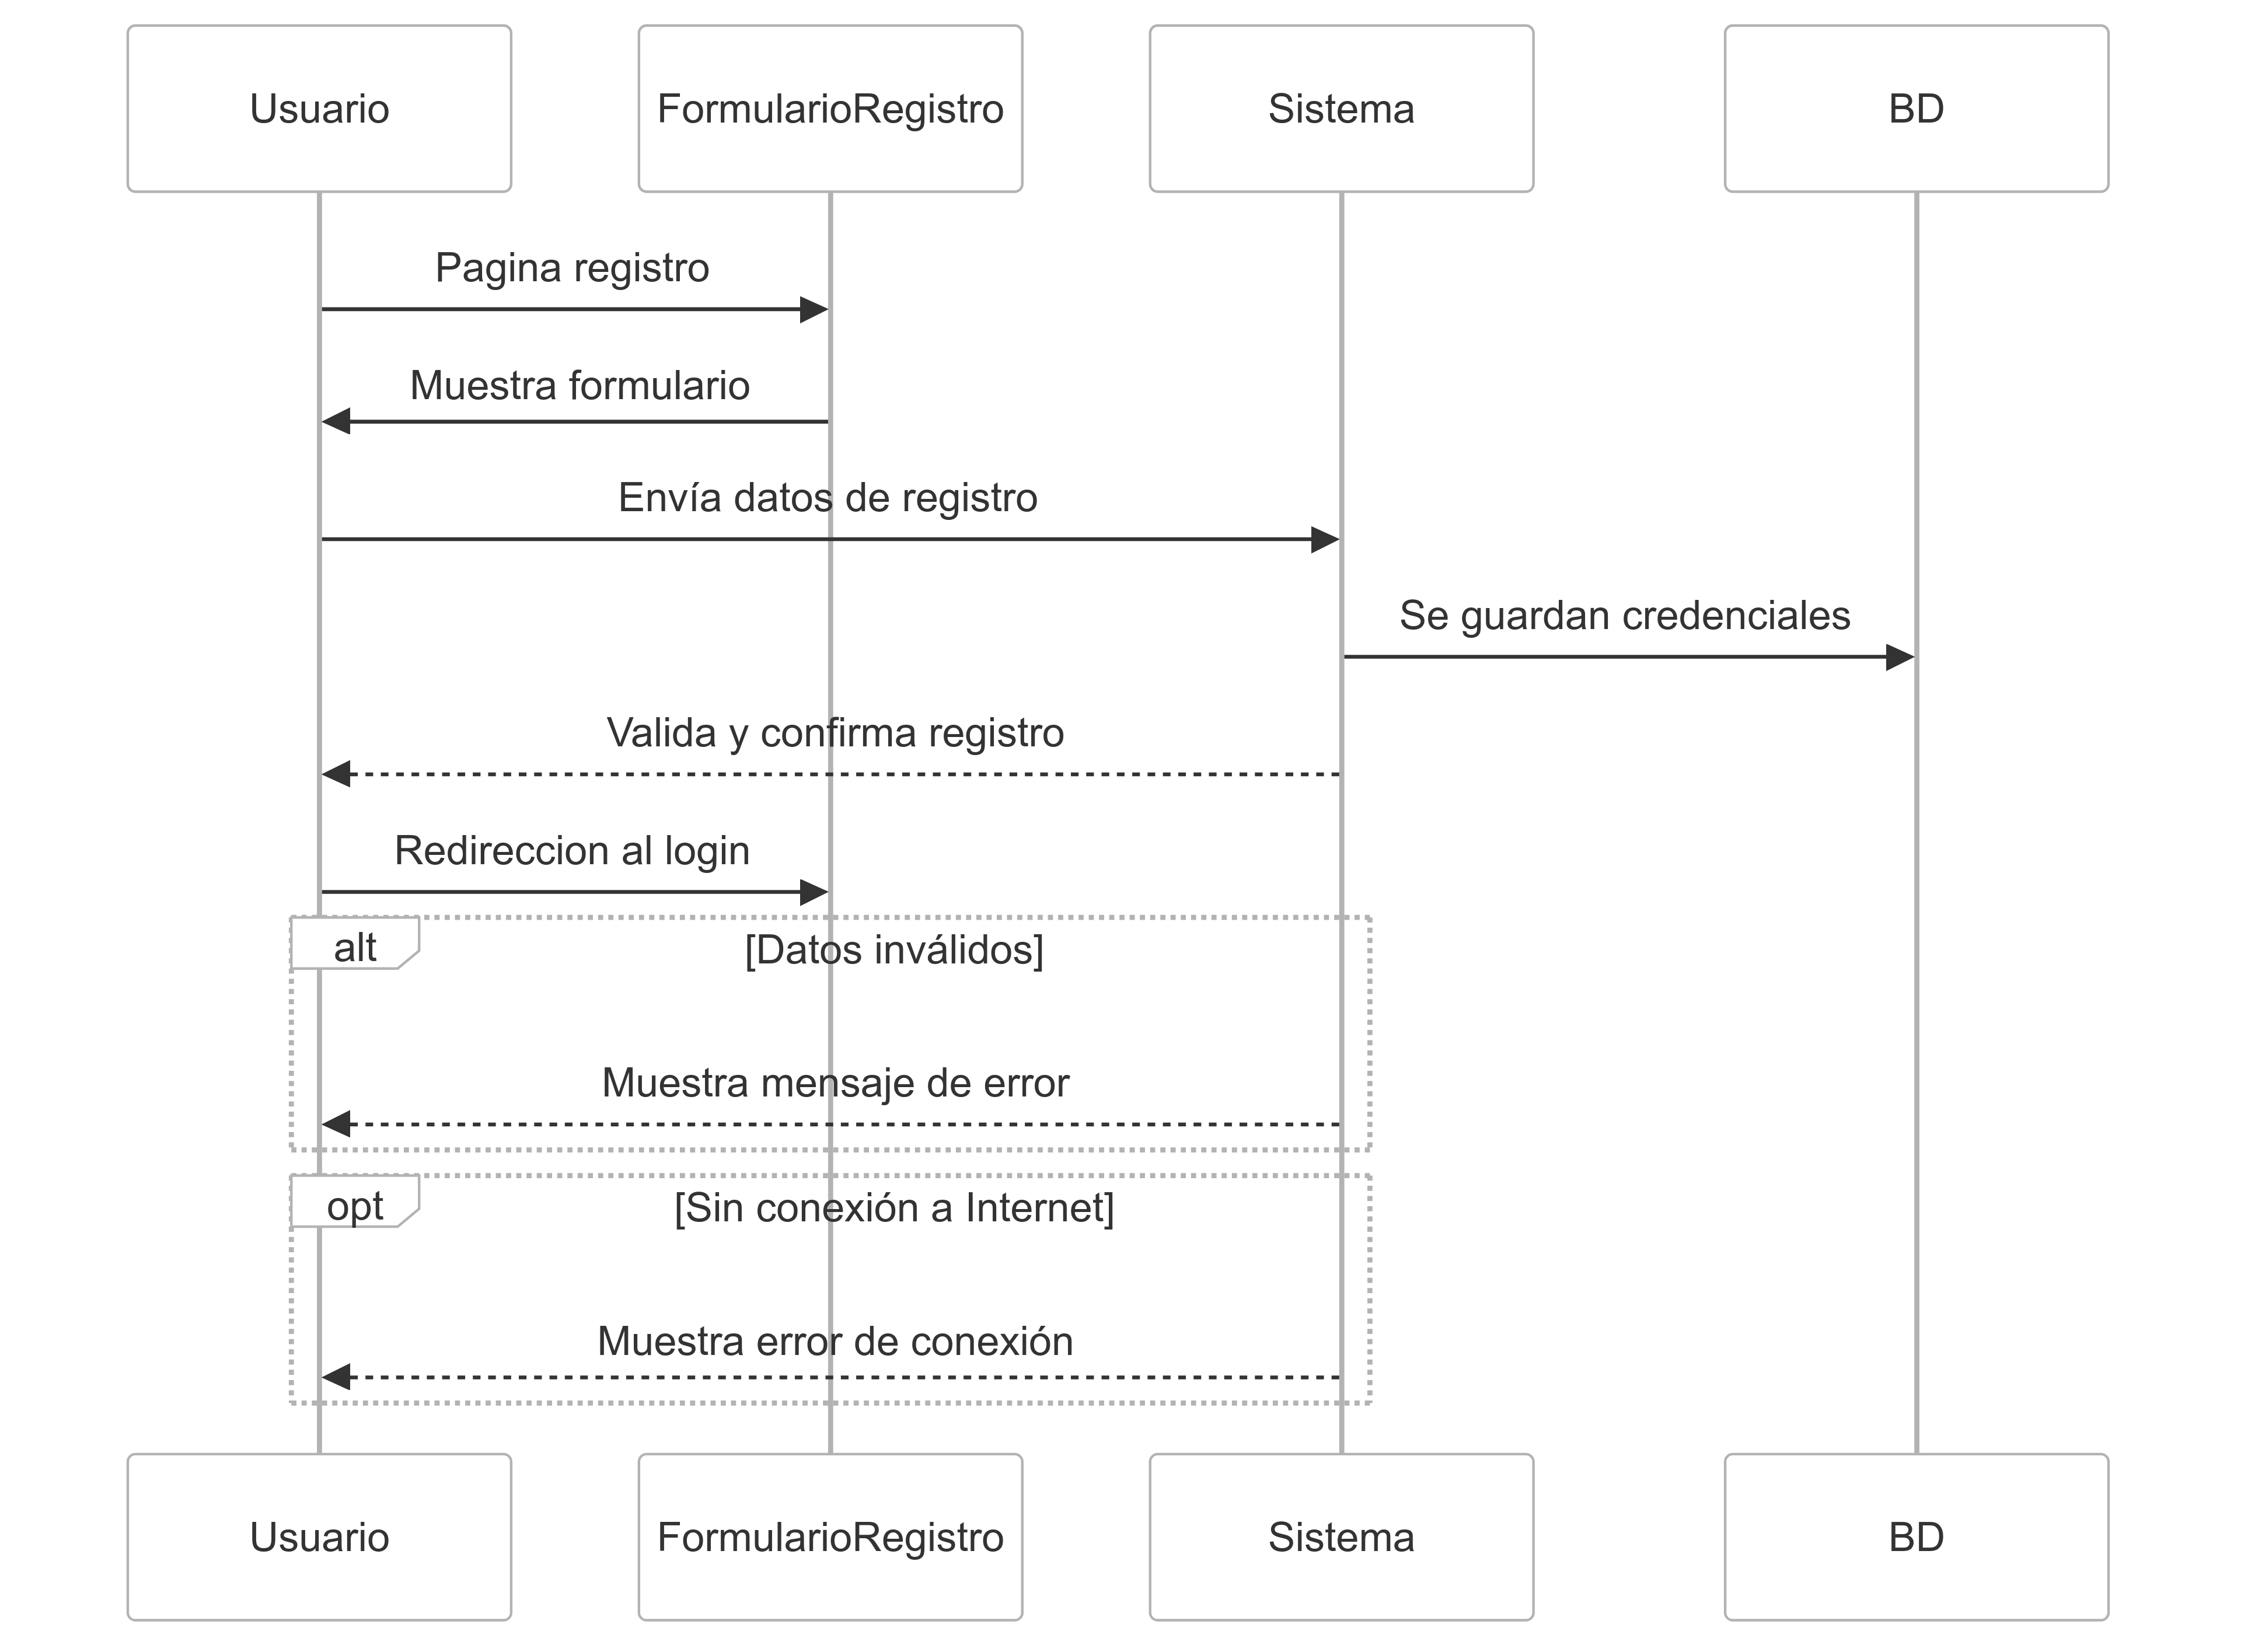
\includegraphics[width=0.5\textwidth]{txt/cu1.png} % Adjust width as needed
    \caption{CU1: Registro}
    \label{fig: 1}
\end{figure} 

\begin{figure}[h]
    \centering
    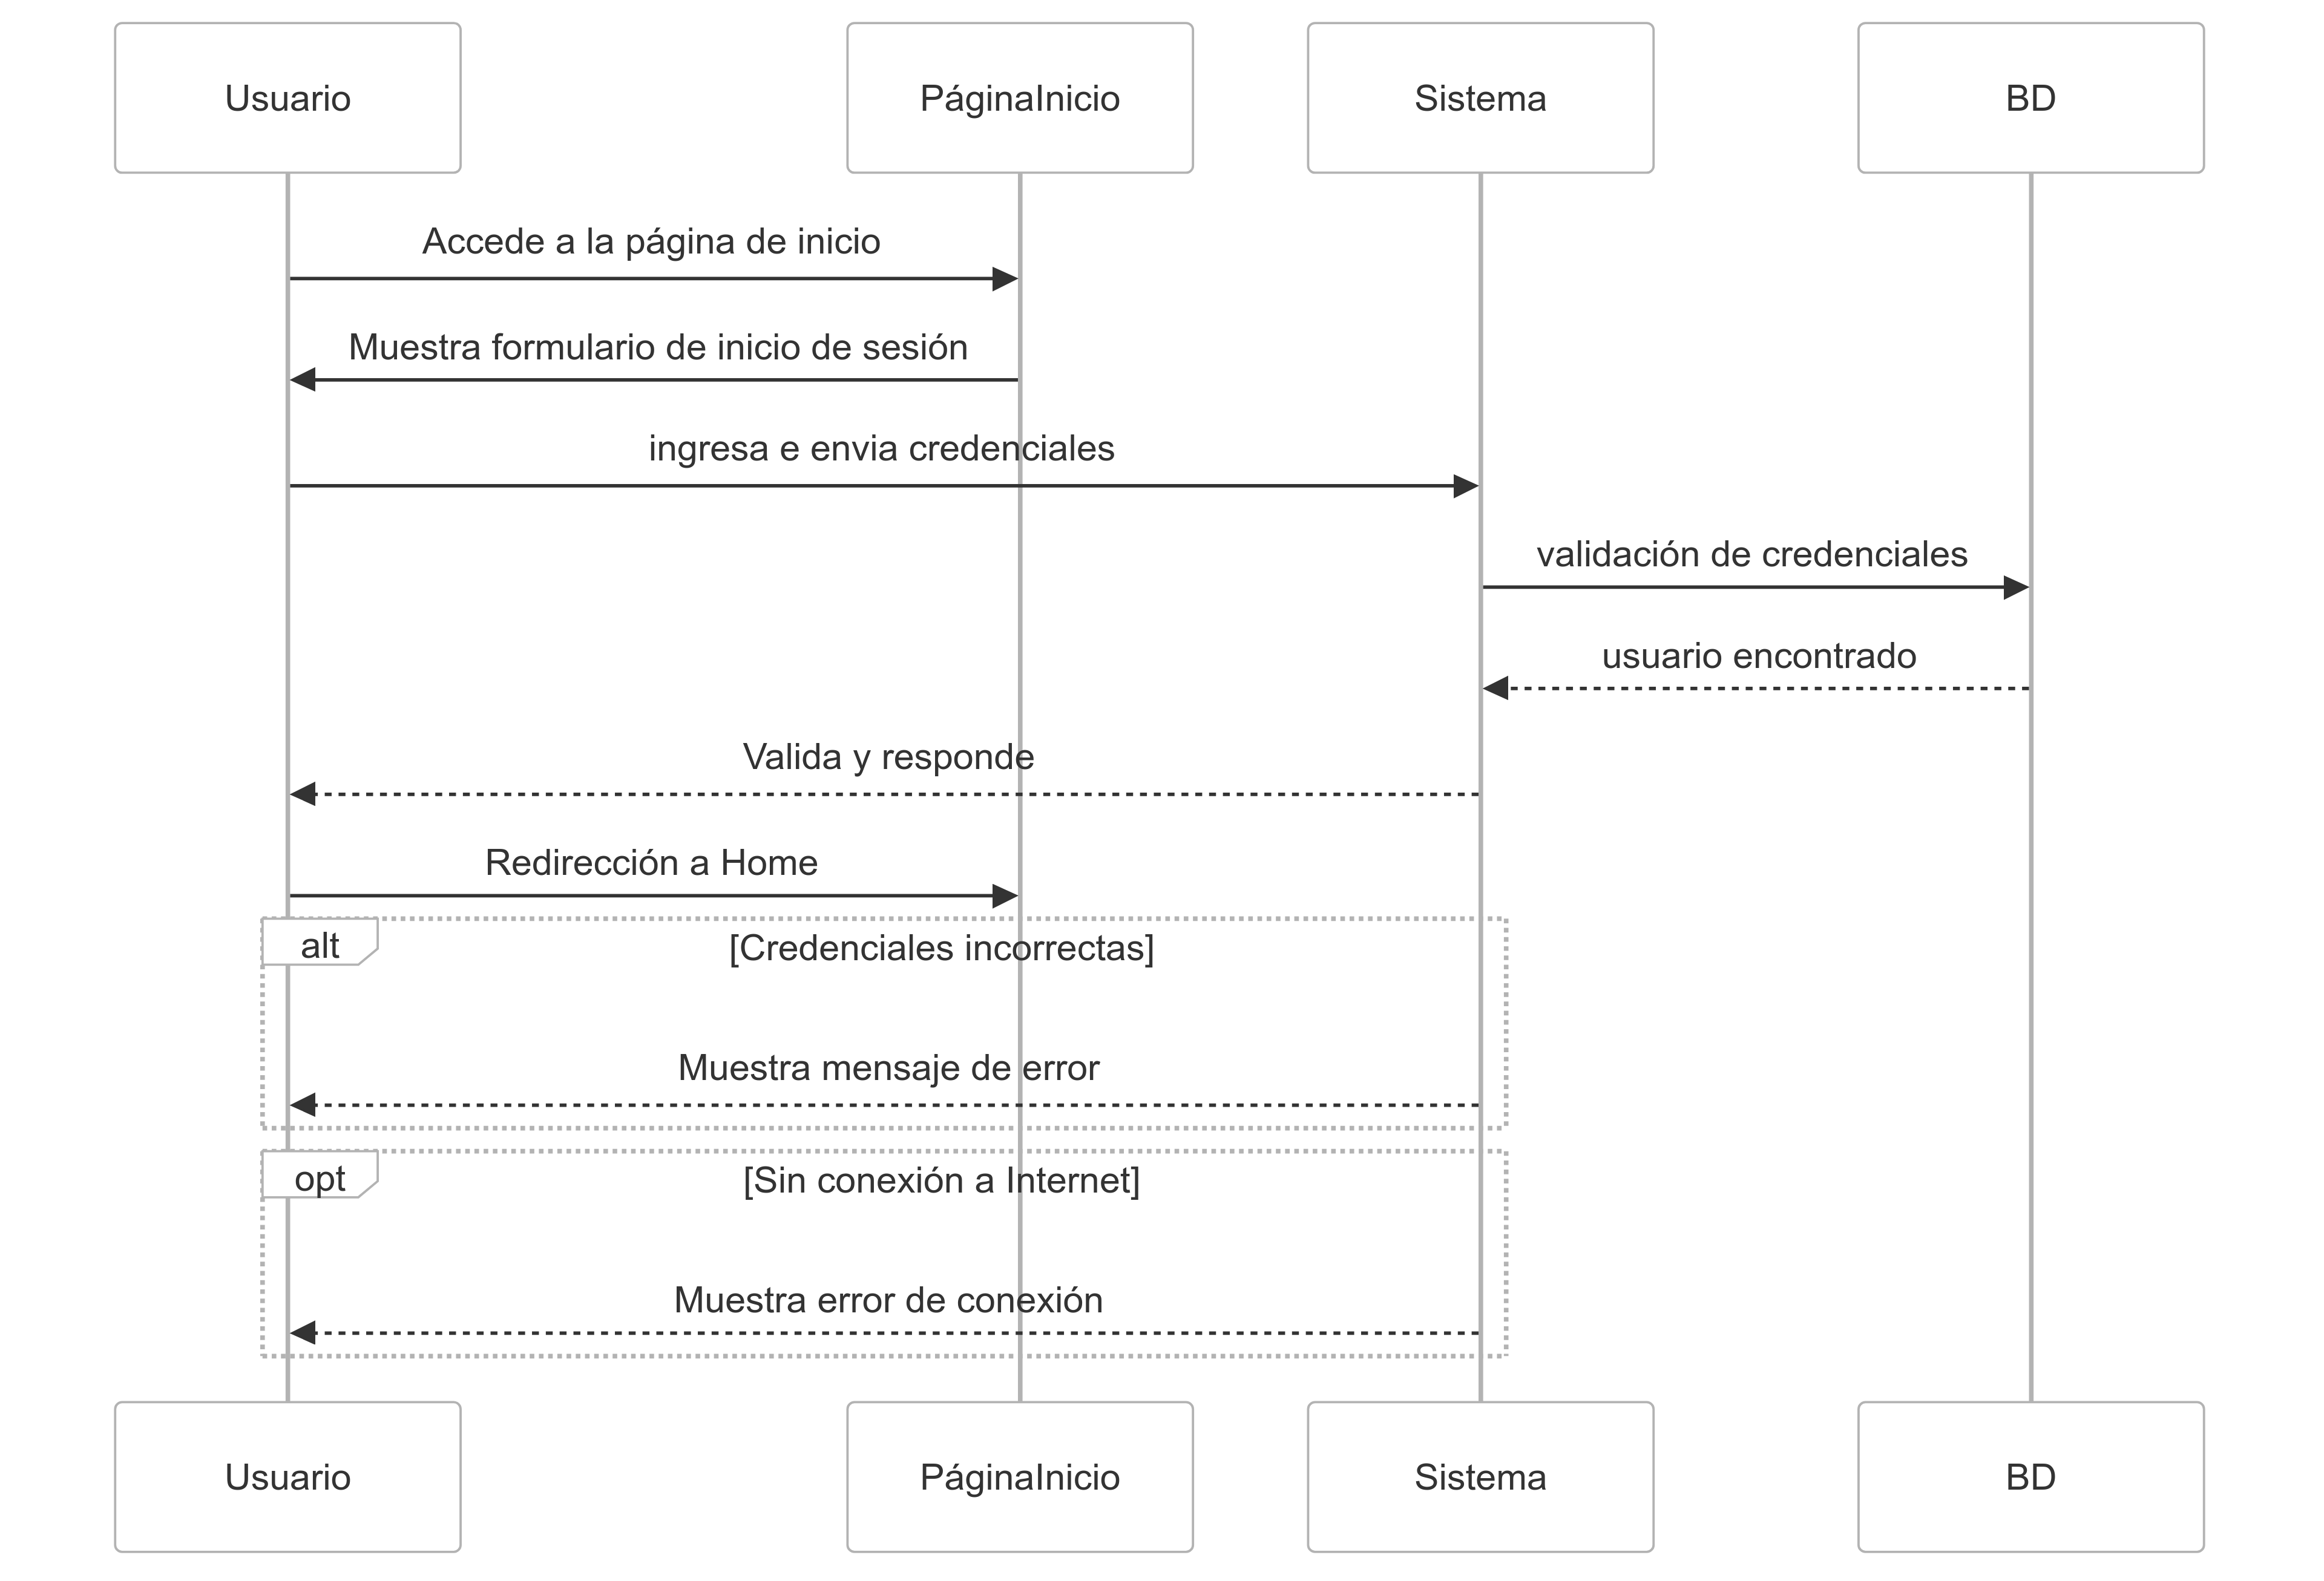
\includegraphics[width=0.5\textwidth]{txt/cu2.png} % Adjust width as needed
    \caption{CU1: Inicio de Sesión}
    \label{fig: 1}
\end{figure}

\begin{figure}[h]
    \centering
    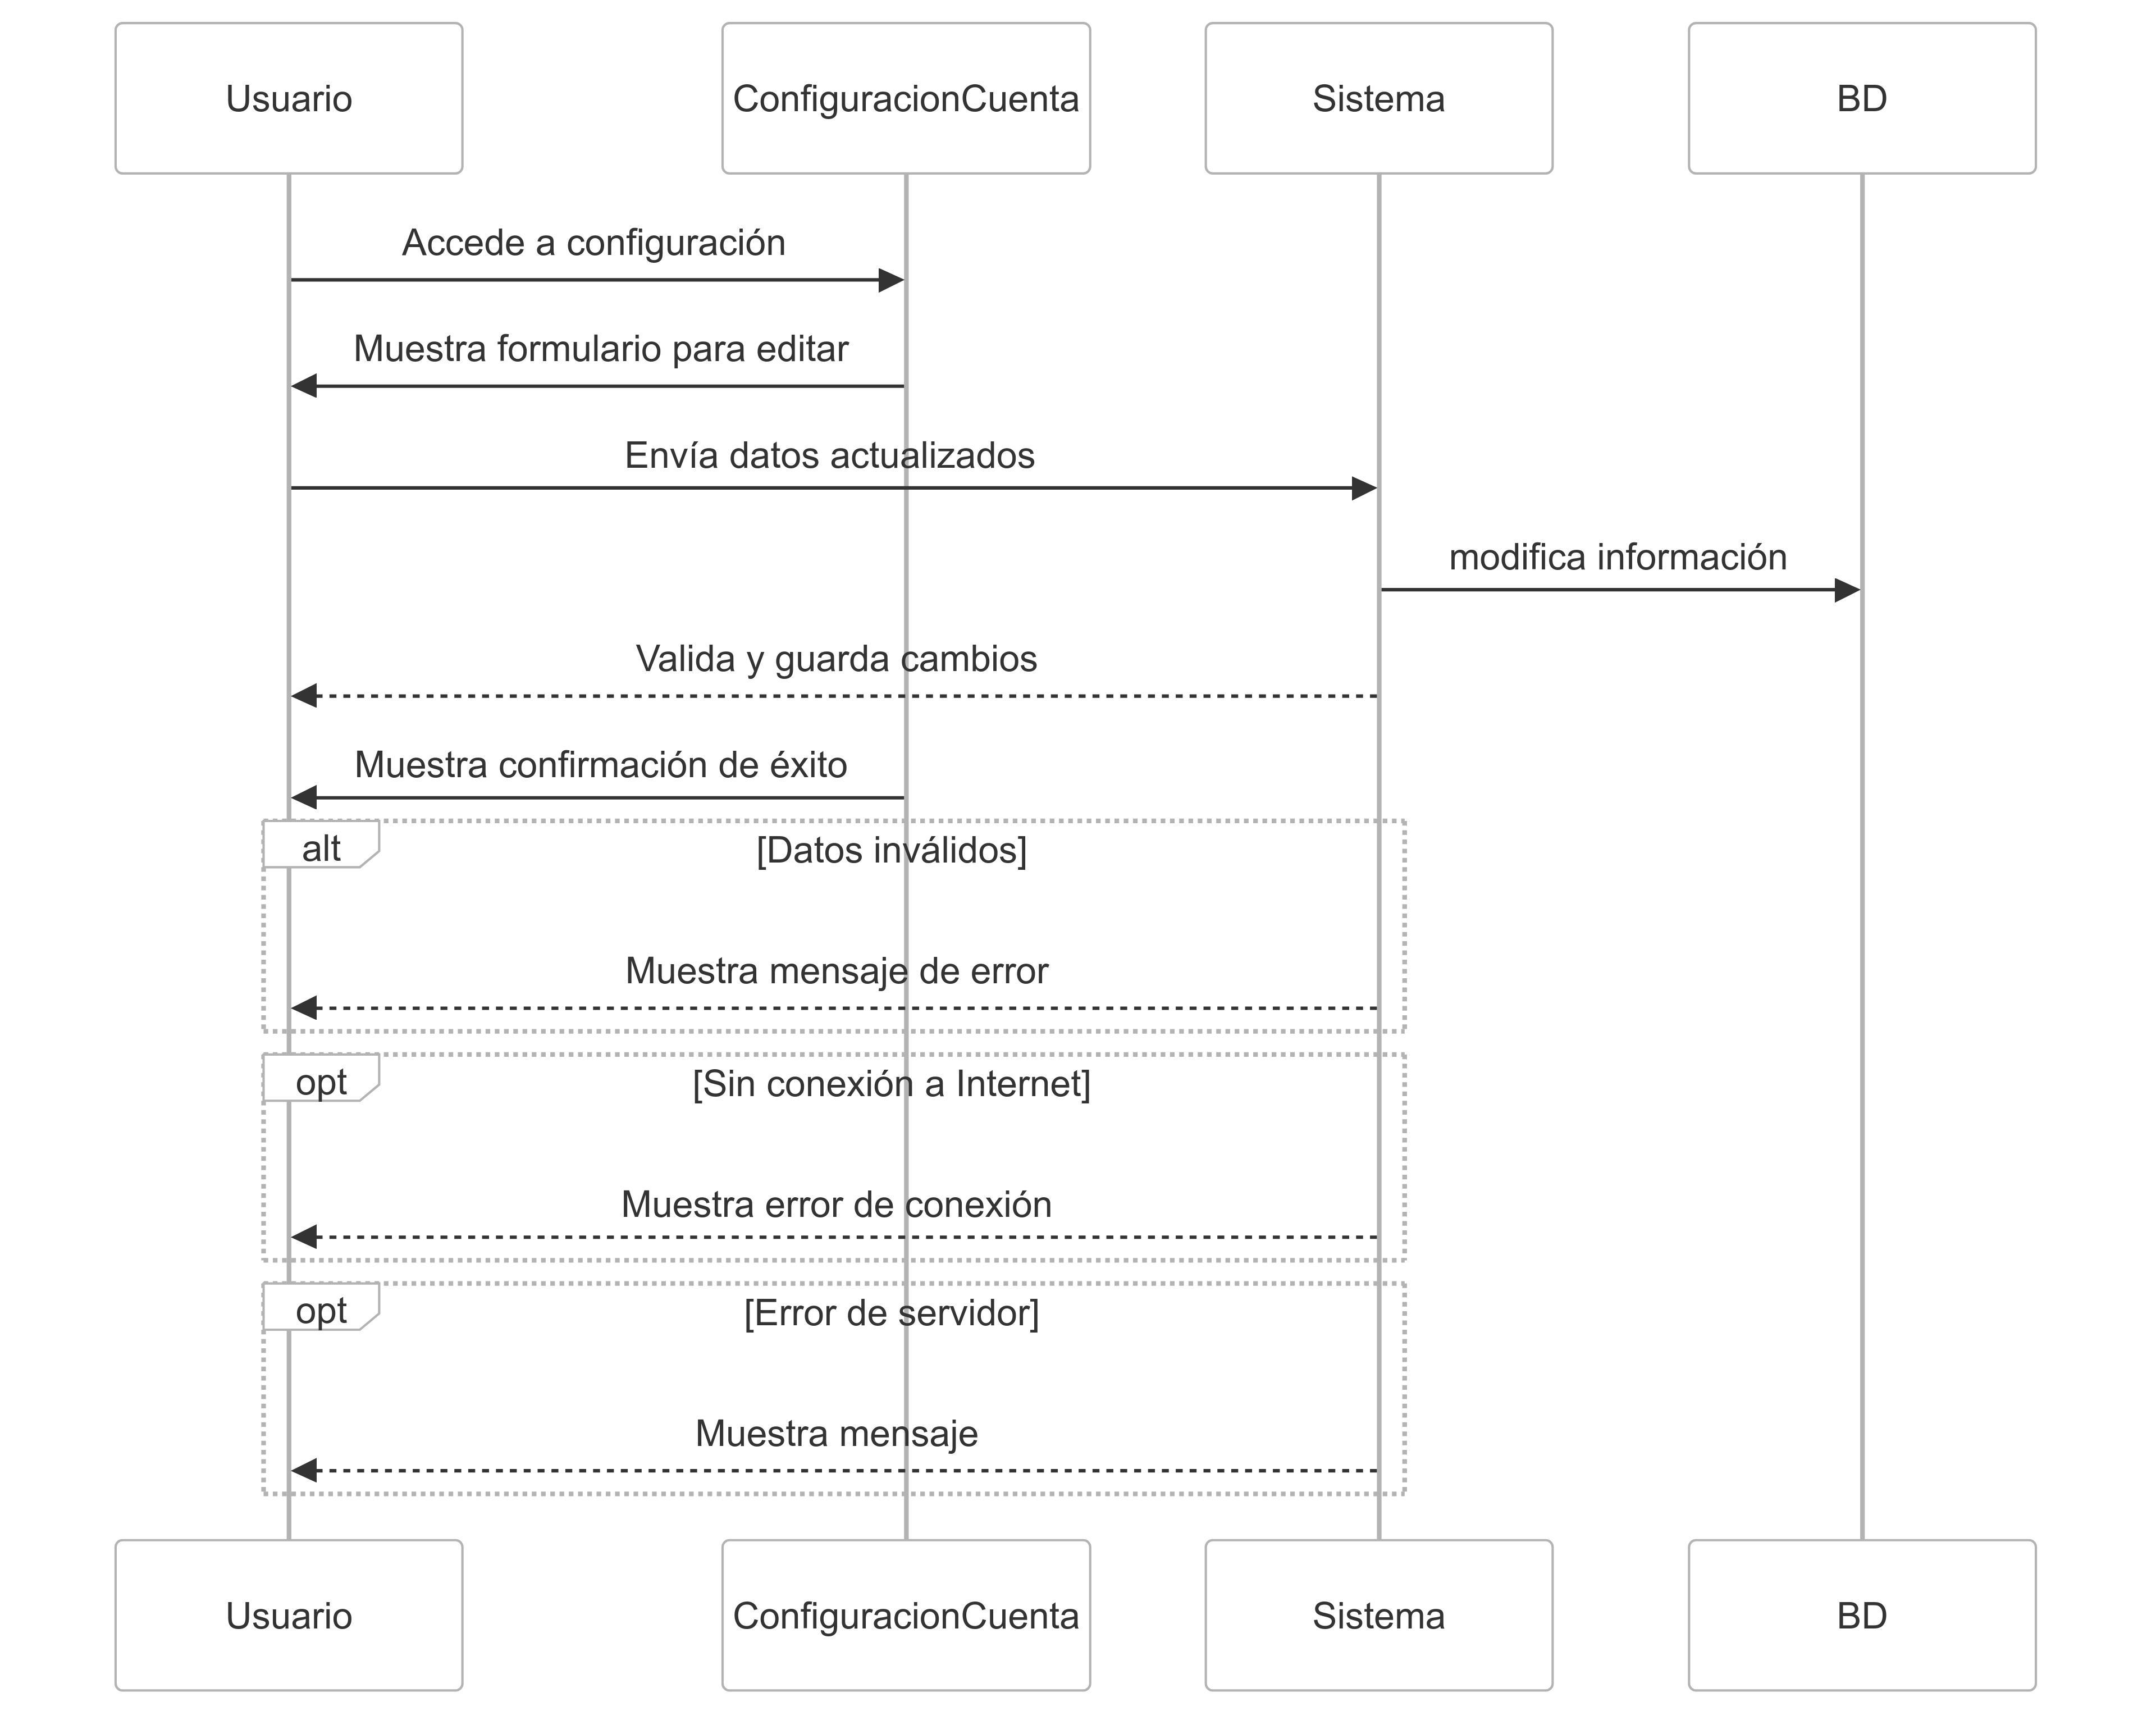
\includegraphics[width=0.5\textwidth]{txt/cu3.png} % Adjust width as needed
    \caption{CU3: Editar datos}
    \label{fig: 1}
\end{figure}




